\documentclass{standalone}
\usepackage{tikz}
\usetikzlibrary{patterns, positioning}


\begin{document}
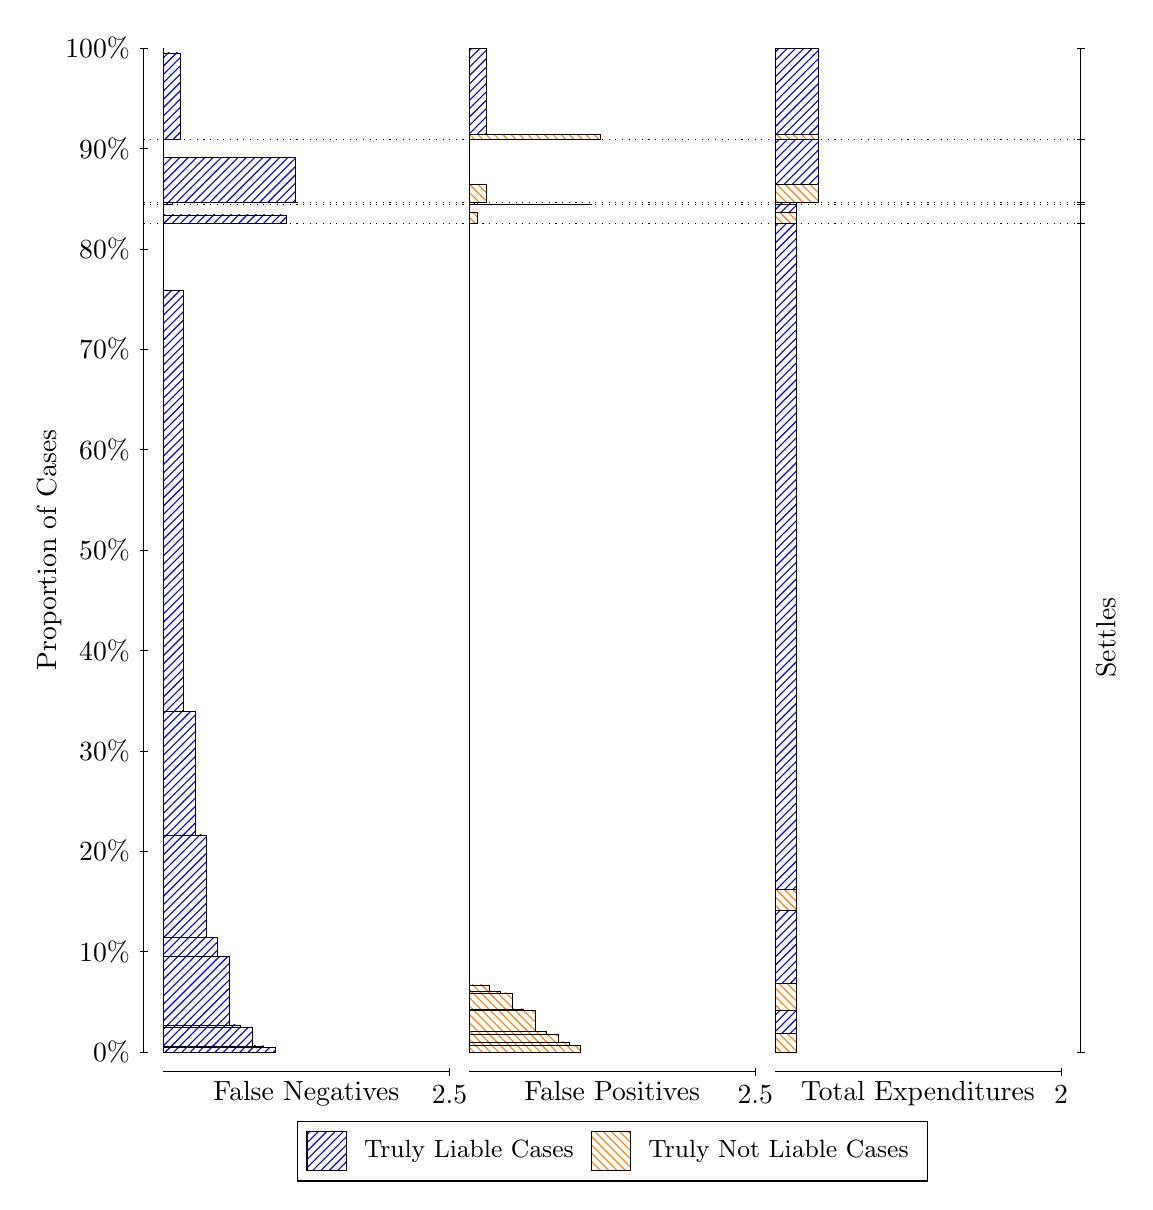
\begin{tikzpicture}
\draw[black, very thin] (1.5,1.75) -- (1.5,14.5);
\node[rotate=90, text=black, anchor=center] at (0.3, 8.125) {Proportion of Cases};
\draw[black, very thin] (1.45,1.75) -- (1.55,1.75);
\node[text=black, anchor=east] at (1.45, 1.75) {0\%};
\draw[black, very thin] (1.45,3.025) -- (1.55,3.025);
\node[text=black, anchor=east] at (1.45, 3.025) {10\%};
\draw[black, very thin] (1.45,4.3) -- (1.55,4.3);
\node[text=black, anchor=east] at (1.45, 4.3) {20\%};
\draw[black, very thin] (1.45,5.575) -- (1.55,5.575);
\node[text=black, anchor=east] at (1.45, 5.575) {30\%};
\draw[black, very thin] (1.45,6.85) -- (1.55,6.85);
\node[text=black, anchor=east] at (1.45, 6.85) {40\%};
\draw[black, very thin] (1.45,8.125) -- (1.55,8.125);
\node[text=black, anchor=east] at (1.45, 8.125) {50\%};
\draw[black, very thin] (1.45,9.4) -- (1.55,9.4);
\node[text=black, anchor=east] at (1.45, 9.4) {60\%};
\draw[black, very thin] (1.45,10.675) -- (1.55,10.675);
\node[text=black, anchor=east] at (1.45, 10.675) {70\%};
\draw[black, very thin] (1.45,11.95) -- (1.55,11.95);
\node[text=black, anchor=east] at (1.45, 11.95) {80\%};
\draw[black, very thin] (1.45,13.225) -- (1.55,13.225);
\node[text=black, anchor=east] at (1.45, 13.225) {90\%};
\draw[black, very thin] (1.45,14.5) -- (1.55,14.5);
\node[text=black, anchor=east] at (1.45, 14.5) {100\%};

\draw[black, very thin] (13.4,1.75) -- (13.4,14.5);
\draw[black, very thin] (13.35,1.75) -- (13.45,1.75);
\node[anchor=west] at (13.35, 1.75) {};
\draw[black, very thin] (13.35,12.277) -- (13.45,12.277);
\node[anchor=west] at (13.35, 12.277) {};
\draw[black, very thin] (13.35,12.514) -- (13.45,12.514);
\node[anchor=west] at (13.35, 12.514) {};
\draw[black, very thin] (13.35,12.542) -- (13.45,12.542);
\node[anchor=west] at (13.35, 12.542) {};
\draw[black, very thin] (13.35,13.34) -- (13.45,13.34);
\node[anchor=west] at (13.35, 13.34) {};
\draw[black, very thin] (13.35,14.5) -- (13.45,14.5);
\node[anchor=west] at (13.35, 14.5) {};

\draw[black, very thin, pattern color=blue, pattern=north east lines] (1.75,1.75) rectangle (3.167,1.8087);
\draw[black, very thin, pattern color=blue, pattern=north east lines] (1.75,1.8087) rectangle (3.0217,1.8271);
\draw[black, very thin, pattern color=blue, pattern=north east lines] (1.75,1.8271) rectangle (2.8763,2.0617);
\draw[black, very thin, pattern color=blue, pattern=north east lines] (1.75,2.0617) rectangle (2.731,2.0936);
\draw[black, very thin, pattern color=blue, pattern=north east lines] (1.75,2.0936) rectangle (2.5857,2.9628);
\draw[black, very thin, pattern color=blue, pattern=north east lines] (1.75,2.9628) rectangle (2.4403,3.201);
\draw[black, very thin, pattern color=blue, pattern=north east lines] (1.75,3.201) rectangle (2.295,4.5057);
\draw[black, very thin, pattern color=blue, pattern=north east lines] (1.75,4.5057) rectangle (2.1497,6.0785);
\draw[black, very thin, pattern color=blue, pattern=north east lines] (1.75,6.0785) rectangle (2.0043,11.425);
\draw[black, very thin, pattern color=orange, pattern=north west lines] (1.75,11.425) rectangle (1.75,12.277);
\draw[black, very thin, pattern color=blue, pattern=north east lines] (1.75,12.277) rectangle (3.3123,12.38);
\draw[black, very thin, pattern color=orange, pattern=north west lines] (1.75,12.38) rectangle (1.75,12.514);
\draw[black, very thin, pattern color=blue, pattern=north east lines] (1.75,12.514) rectangle (1.859,12.541);
\draw[black, very thin, pattern color=orange, pattern=north west lines] (1.75,12.541) rectangle (1.75,12.542);
\draw[black, very thin, pattern color=blue, pattern=north east lines] (1.75,12.542) rectangle (3.4213,13.115);
\draw[black, very thin, pattern color=orange, pattern=north west lines] (1.75,13.115) rectangle (1.75,13.34);
\draw[black, very thin, pattern color=blue, pattern=north east lines] (1.75,13.34) rectangle (1.968,14.437);
\draw[black, very thin, pattern color=orange, pattern=north west lines] (1.75,14.437) rectangle (1.75,14.5);
\draw[black, very thin, pattern color=orange, pattern=north west lines] (5.6333,1.75) rectangle (7.0503,1.8345);
\draw[black, very thin, pattern color=orange, pattern=north west lines] (5.6333,1.8345) rectangle (6.905,1.8776);
\draw[black, very thin, pattern color=orange, pattern=north west lines] (5.6333,1.8776) rectangle (6.7597,1.9737);
\draw[black, very thin, pattern color=orange, pattern=north west lines] (5.6333,1.9737) rectangle (6.6143,2.0122);
\draw[black, very thin, pattern color=orange, pattern=north west lines] (5.6333,2.0122) rectangle (6.469,2.2801);
\draw[black, very thin, pattern color=orange, pattern=north west lines] (5.6333,2.2801) rectangle (6.3237,2.297);
\draw[black, very thin, pattern color=orange, pattern=north west lines] (5.6333,2.297) rectangle (6.1783,2.5018);
\draw[black, very thin, pattern color=orange, pattern=north west lines] (5.6333,2.5018) rectangle (6.033,2.5207);
\draw[black, very thin, pattern color=orange, pattern=north west lines] (5.6333,2.5207) rectangle (5.8877,2.6021);
\draw[black, very thin, pattern color=blue, pattern=north east lines] (5.6333,2.6021) rectangle (5.6333,12.277);
\draw[black, very thin, pattern color=orange, pattern=north west lines] (5.6333,12.277) rectangle (5.7423,12.41);
\draw[black, very thin, pattern color=blue, pattern=north east lines] (5.6333,12.41) rectangle (5.6333,12.514);
\draw[black, very thin, pattern color=orange, pattern=north west lines] (5.6333,12.514) rectangle (7.1957,12.514);
\draw[black, very thin, pattern color=blue, pattern=north east lines] (5.6333,12.514) rectangle (5.7423,12.542);
\draw[black, very thin, pattern color=orange, pattern=north west lines] (5.6333,12.542) rectangle (5.8513,12.768);
\draw[black, very thin, pattern color=blue, pattern=north east lines] (5.6333,12.768) rectangle (5.6333,13.34);
\draw[black, very thin, pattern color=orange, pattern=north west lines] (5.6333,13.34) rectangle (7.3047,13.403);
\draw[black, very thin, pattern color=blue, pattern=north east lines] (5.6333,13.403) rectangle (5.8513,14.5);
\draw[black, very thin, pattern color=orange, pattern=north west lines] (9.5167,1.75) rectangle (9.7892,1.9907);
\draw[black, very thin, pattern color=blue, pattern=north east lines] (9.5167,1.9907) rectangle (9.7892,2.2756);
\draw[black, very thin, pattern color=orange, pattern=north west lines] (9.5167,2.2756) rectangle (9.7892,2.6247);
\draw[black, very thin, pattern color=blue, pattern=north east lines] (9.5167,2.6247) rectangle (9.7892,3.5526);
\draw[black, very thin, pattern color=orange, pattern=north west lines] (9.5167,3.5526) rectangle (9.7892,3.8148);
\draw[black, very thin, pattern color=blue, pattern=north east lines] (9.5167,3.8148) rectangle (9.7892,12.277);
\draw[black, very thin, pattern color=orange, pattern=north west lines] (9.5167,12.277) rectangle (9.7892,12.41);
\draw[black, very thin, pattern color=blue, pattern=north east lines] (9.5167,12.41) rectangle (9.7892,12.514);
\draw[black, very thin, pattern color=orange, pattern=north west lines] (9.5167,12.514) rectangle (9.7892,12.514);
\draw[black, very thin, pattern color=blue, pattern=north east lines] (9.5167,12.514) rectangle (9.7892,12.542);
\draw[black, very thin, pattern color=orange, pattern=north west lines] (9.5167,12.542) rectangle (10.062,12.768);
\draw[black, very thin, pattern color=blue, pattern=north east lines] (9.5167,12.768) rectangle (10.062,13.34);
\draw[black, very thin, pattern color=orange, pattern=north west lines] (9.5167,13.34) rectangle (10.062,13.403);
\draw[black, very thin, pattern color=blue, pattern=north east lines] (9.5167,13.403) rectangle (10.062,14.5);
\draw[black, dotted] (1.5,12.277) -- (13.4,12.277);
\draw[black, dotted] (1.5,12.514) -- (13.4,12.514);
\draw[black, dotted] (1.5,12.542) -- (13.4,12.542);
\draw[black, dotted] (1.5,13.34) -- (13.4,13.34);
\draw[black, very thin] (1.75,1.5) -- (5.3833,1.5);
\node[text=black, anchor=north] at (3.5667, 1.5) {False Negatives};
\draw[black, very thin] (5.3833,1.45) -- (5.3833,1.55);
\node[text=black, anchor=north] at (5.3833, 1.45) {2.5};

\draw[black, very thin] (5.6333,1.5) -- (9.2667,1.5);
\node[text=black, anchor=north] at (7.45, 1.5) {False Positives};
\draw[black, very thin] (9.2667,1.45) -- (9.2667,1.55);
\node[text=black, anchor=north] at (9.2667, 1.45) {2.5};

\draw[black, very thin] (9.5167,1.5) -- (13.15,1.5);
\node[text=black, anchor=north] at (11.333, 1.5) {Total Expenditures};
\draw[black, very thin] (13.15,1.45) -- (13.15,1.55);
\node[text=black, anchor=north] at (13.15, 1.45) {2};

\node[text=black, centered, rotate=90] at (13.72, 7.0134) {Settles};





\draw (7.449999999999999,1.5) node[draw=none] (baseCoordinate) {};
\begin{scope}[align=center]
        \matrix[scale=0.5, draw=black, below=0.5cm of baseCoordinate, nodes={draw}, column sep=0.1cm]{
            \node[rectangle, draw, minimum width=0.5cm, minimum height=0.5cm, pattern color=blue, pattern=north east lines] {}; &
            \node[draw=none, font=\small, text=black] (B) {Truly Liable Cases}; &
            \node[rectangle, draw, minimum width=0.5cm, minimum height=0.5cm, pattern color=orange, pattern=north west lines] {}; &
            \node[draw=none, font=\small, text=black] (B) {Truly Not Liable Cases}; \\
            };
\end{scope}

\end{tikzpicture}
\end{document}